
\section{Local connectivity and q-tameness} \label{s:connectivity}

Let $\H$ be a fixed homology theory.

\begin{defi} \label{defi:local_connectedness}
	For $n \in \Z$ a continuous map is said to be \textit{$n$-homologically small} or \textit{trivial}, denoted $\HS_n$ and $\HT_n$ respectively, if the image of the map induced by $\H_n$ is finitely generated or 0, and we say it is \textit{homologically small} or \textit{trivial}, denoted respectively $\HS$ and $\HT$, if it is $\HS_n$ or $\HT_n$ for every~$n$.
\end{defi}

\begin{defi}
	A space $X$ is said to be \emph{homologically locally connected}, denoted $\HLC$, if for each $x \in X$ any neighborhood $V$ of $x$ contains a neighborhood $U$ of $x$ such that the inclusion $U \to V$ is $\HT$.
\end{defi}

Local connectivity assumptions have a long history of being used to ensure that different homology theories agree and to ensure that homology is finite dimensional.
We mention the following examples.

Recall that a space is said to be \textit{paracompact} if every open cover has a locally finite open refinement, i.e., every point has a neighborhood intersecting finitely many sets in the refinement.
\begin{prop}[\cite{MR105677}] \label{prop:cech_sing_hom_hlc}
	\v{C}ech and singular homology with arbitrary coefficients coincide on the category of paracompact Hausdorff spaces which are $\HLC$ with respect to integral singular homology.
\end{prop}

\begin{prop} \label{prop:fin_dim_sing_hom}
	Let $X$ be a compact Hausdorff space.
	If $X$ is $\HLC$ with respect to integral singular homology, then the singular homology of $X$ with arbitrary coefficients is finite-dimensional in every degree.
\end{prop}

We will deduce the previous finiteness result from our main contribution, Theorem~\ref{t:strong local connectenss implies q-tameness}.
To motivate the statement of our theorem let us record a direct consequence of the previous proposition.

\begin{prop}
	Let $(X, f)$ be a sublevel filtration. If each sublevel set is compact and $\HLC$ with respect to integral singular homology, then its singular persistence module is p.f.d. in every degree, in particular q-tame.
\end{prop}

Having each sublevel set being $\HLC$ is in many cases too restrictive.
We would like a relative condition for sublevel filtrations to be sufficient to ensure the q-tameness of the associated persistence module.
The following definitions are motivated by Morse's work, please consult Section~\ref{s:historical} for their relation to his original statements. 

\begin{defi} \label{defi:local_connectedness_filtrations}
	For a fix homology theory $\H$. A sublevel filtration $(X,f)$ is said to be $\HLC$ if for any $\epsilon > 0$, $x \in X$, and $V$ an open neighborhood of $x$, there is a $\delta \in (0, \epsilon)$ and a neighborhood $U$ of $x$ such that $U \subseteq V$ and
	\begin{equation*}
	X_{\leq f(x) + \delta + c} \cap U \to X_{\leq f(x) + \epsilon + c} \cap V
	\end{equation*}
	is $\HT$ for every $c \geq 0$.
	We also consider a weaker version, referred to as \textit{weakly} $\HLC$, defined as above with $c = 0$.
\end{defi}

We will now show that the weak notion does not imply q-tameness in general.
To do so let us consider the \textit{$d$-dimensional Hawaiian earring}
\begin{equation*}
\HE = \bigcup_{n\in\mathbb{N}}\left\{(x_0,\dots,x_d)\in\R^{d+1} \ \middle | \ \left(x_0-\frac{1}{n}\right)^2+x_1^2+\dots+x_d^2=\left(\frac{1}{n}\right)^2\right\}.
\end{equation*}

\begin{figure}[t]
	\centering
	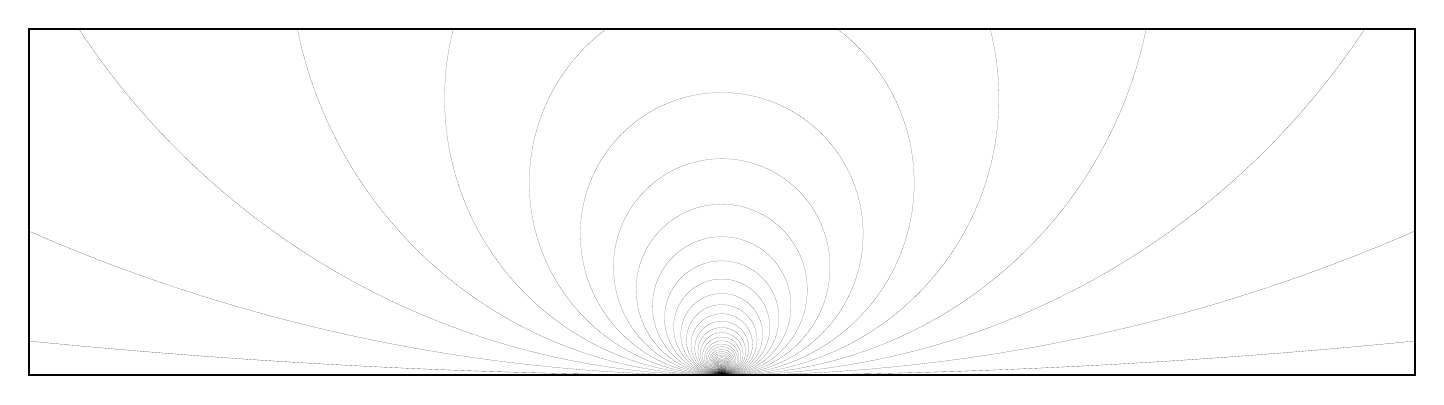
\begin{tikzpicture}[scale=88]
	\draw[thick] (-.1,0) rectangle (.1,.05);
	\clip (-.1,0) rectangle (.1,.05); % remove for all circles
	\foreach \i in {1,...,100}{
		\draw[line width=0.1/\i mm] (0, 1/\i^2) circle (1/\i^2);
	}
	\end{tikzpicture}
	\caption{A closeup of the Hawaiian earring $\mathbb{H}^1$.}
	\label{fig:earrings}
\end{figure}

\begin{thm} \label{thm:counterexample}
	Let $\H$ be a (generalized) homology theory such that its value on a point is finitely generated for every degree and on $\HE$ is not finitely generated for some degree. Then, the function $f \colon \HE \to \R$ whose value at the origin is $0$ and is $1$ everywhere else defines a weakly $\HLC$ Morse filtration that is not q-tame.
\end{thm}

\begin{proof}
	The space $\HE$ is Hausdorff and locally compact since $R^{d+1}$ is.
	To verify that $(\HE,f)$ is a Morse filtration we notice that all level sets are either the empty set, the singleton containing the origin, or $\HE$ itself, all compact spaces.
	Let us now verify that $\HE$ is $\HLC$.
	Let $\epsilon > 0$ and $x \in \HE$.
	If $x$ is the origin, we choose $\delta$ between $0$ and the minimum of $\epsilon$ and $1$.
	Then $\HE_{\leq f(x) + \delta} = \HE_{\leq \delta} = \{x\}$, so the desired condition follows from the first assumption on the homology theory.
	For $x$ not the origin, there is a unique $d$-sphere that contains it.
	Clearly, we may choose $\delta > 0$ so small that $D_\delta(x) = \{y \in \R^{d+1} \mid \Vert x - y \Vert < \delta\} \cap \HE$ is contained in this sphere, so $D_\delta(x)$ is homotopy equivalent to a $x$ and the condition again follows trivially.
	What remains to be shown is that $\HE_{\leq \bullet}$ is not q-tame.
	Since $\HE_{\leq t}$ is constant with value $\HE$ for $t \geq 1$, the second assumption on the homology theory finishes the proof.
\end{proof}

The theories that we are most interested in do satisfy these conditions.

\begin{prop}
	The assumptions of Theorem~\ref{thm:counterexample} are satisfied by singular homology with arbitrary coefficients and \v{Cech} homology with field coefficients.
\end{prop}

\begin{proof}
	The case of singular homology is well know and can be found in \cite{Barratt.1962}.
	For \v{C}ech homology we use the fact that it commutes with inverse limits for compact Hausdorff spaces.
	Define 
	\begin{align*}
	\HE_k &= \left\{(x_0,\dots,x_d)\in\R^{d+1}\mid \left(x_0-\frac{1}{k}\right)^2+x_1^2+\dots+x_d^2 \leq \left(\frac{1}{k}\right)^2\right\}\\
	&\cup\bigcup_{n=1}^{k-1}\left\{(x_0,\dots,x_d)\in\R^{d+1}\mid \left(x_0-\frac{1}{n}\right)^2+x_1^2+\dots+x_d^2=\left(\frac{1}{n}\right)^2\right\},
	\end{align*}
	i.e., the $d$-dimensional Hawaiian earring but with the $k$-th largest $d$-sphere filled.
	We have $\lim_{k}\HE_{k} = \bigcap_{k}\mathbb{H}^{d}_{k}=\mathbb{H}^{d}$, and hence $\CH_{d}(\HE) = \lim_{k}\CH_{d}(\mathbb{H}^{d}_{k})$.
	Each $\mathbb{H}^{d}_{k}$ is a CW-complex, so we can simply use cellular homology to compute
	\begin{equation*}
	\lim_{k}\CH_{d}(\mathbb{H}^{d}_{k})=\lim\left(\dots\to \prod_{n=1}^2\mathbb{F}\to \prod_{n=1}^1\mathbb{F}\to \prod_{n=1}^0\mathbb{F}\right)=\prod_{n\in\mathbb{N}}\mathbb{F},
	\end{equation*}
	which is infinite-dimensional over $\mathbb{F}$.
	This finishes the proof.
\end{proof}

Now we verify that Morse filtrations which are $\HLC$ are q-tame.
We will need three lemmas. 

\begin{lem} \label{l:commutative algebra}
	Given a commutative diagram of modules over a principal ideal domain
	\begin{equation*}
	\begin{tikzcd}
	A_{1,1} \arrow[r] & A_{1,2} & \\
	A_{2,1} \arrow[r] \arrow[u] & A_{2,2} \arrow[r] \arrow[u] & A_{2,3} \\
	& A_{3,2} \arrow[r] \arrow[u] & A_{3,3} \arrow[u]
	\end{tikzcd}
	\end{equation*}
	where the middle row is exact and both $A_{2,1} \to A_{1,1}$ and $A_{3,3} \to A_{2,3}$ have finitely generated images, then so does $A_{3,2} \to A_{1,2}$.
\end{lem}

\begin{proof}
	This is proven via a straightforward diagram chase. For more details see Lemma 17.3 in \cite{Bredon.1968}.
\end{proof}

\begin{lem} \label{l:neighborhood third}
	Let $X$ be locally compact space.
	For any compact subset $K$ and open set $U$ with $K \subseteq U$ there exists a compact set $K^\prime$ such that
	\begin{equation*}
	K \subseteq \interior(K^\prime) \subseteq K^\prime \subseteq U.
	\end{equation*}
\end{lem}

\begin{proof}
	For any $x \in K$ choose a compact neighborhood $C(x) \subseteq U$.
	We have
	\begin{equation*}
	K \subseteq \bigcup_K \interior(C(x)) \subseteq \interior\left(\bigcup_K C(x)\right) \subseteq \bigcup_K C(x) \subseteq U
	\end{equation*}
	Since $K$ is compact, the first inclusion above is achieved over a finite subset $\{x_1, \dots, x_m\}$ of elements in $K$.
	Defining $K^\prime = \bigcup_{i=1}^m C(x_i)$ finishes the proof.
\end{proof}

\begin{lem} \label{l:key lemma for q-tameness}
	Fix a homology theory. Let $(X,f)$ be a $\HLC$ Morse filtration.
	Consider sets $K, L \subseteq X$ with $K$ compact and $K \subseteq \interior(L)$. For any $s < t$ there is $\delta \in (0,\, t-s)$ such that $K \cap X_{s+\delta} \to L \cap X_{t}$ is $\HS$.
\end{lem}

\begin{proof}
	We need to prove that the inclusion $X_s \to X_t$ is $\HS$ for every $s < t$.
	
	The lemma holds for $\HS$ replaced by $\HS_{(n-1)}$ for any $n \leq 0$ since $\H_{n-1}$ induces the zero map. We will proceed by induction on $n$ assuming the lemma for $\HS_{(n-1)}$. 
	
	Given a compact set $L \subseteq X$ and $s < t$ let $\Sigma_{s, t}$ be the collection of all compact subsets $K$ of $\interior(L)$ for which there exists $\delta_K > 0$ and an open neighborhood $U(K)$ of $K$ such that $U(K) \cap X_{s+\delta_K} \to L \cap X_{t}$ is $\HS_n$.
	
	We start by showing that any element of $\interior(L) \cap X_s$ has a neighborhood in $\Sigma_{s, t}$.
	Let $x \in \interior(L) \cap X_{s}$.
	Consider an open neighborhood $U(x)$ of $x$ contained in $\interior(L)$, and take $\epsilon > 0$ such that $s + \epsilon < t$.
	By the strong $\HLC$ of $(X,f)$ there is a $\delta \in (0, \epsilon)$ and an open neighborhood $W(x) \subseteq U(x)$ such that for $c = s - f(x)$ the following composition is $\HS$:
	\begin{equation*}
	W(x) \cap X_{f(x) + c + \delta} \to
	U(x) \cap X_{f(x) + c + e} \to
	L \cap X_{t}.
	\end{equation*}
	By local connectivity we can choose a compact neighborhood of $x$ contained in $W(x)$.
	This proves the claim.
	
	We will now show that the class $\Sigma_{s,t}$ is closed under finite unions.
	For $i \in \{1, 2\}$ let $K_i$ be in $\Sigma_{s,t}$ with $\delta_i > 0$ and $K_i \subseteq U_i$ open such that $U_{i} \cap X_{s+\delta_i} \to L \cap X_{t}$ is $\HS_n$.
	We use Lemma \ref{l:neighborhood third} to construct sets $K_i^\prime$ such that
	\begin{equation*}
	K_i \subseteq \interior(K_i^\prime) \subseteq K_i^\prime \subseteq U_i.
	\end{equation*}
	Notice that for $\delta = \min(\delta_i)$ we have $K_i^\prime \cap X_{s+\delta} \to L \cap X_t$ is $\HS_n$.
	Additionally, the induction hypothesis implies that $K_1 \cap K_2 \cap X_s \to K_1^\prime \cap K_2^\prime \cap X_{s+\delta}$ is $\HS_{(n-1)}$.
	We therefore have the following commutative diagram satisfying the assumptions of Lemma~\ref{l:commutative algebra}:\todo{check assumptions for mayer-vietoris to apply}
	\begin{equation*}
	\begin{tikzcd}
	\H_n(L \cap X_t) \oplus \H_n(L \cap X_t) \arrow[r] &
	\H_n(L \cap X_t) & \\
	\H_{n}(K_1^\prime \cap X_{s+\delta}) \oplus \H_n(K_2^\prime \cap X_{s+\delta}) \arrow[r] \arrow[u] & 
	\H_{n}((K_1^\prime \cap X_{s+\delta}) \cup (K_2^\prime \cap X_{s+\delta})) \arrow[r] \arrow[u] &
	\H_{n-1}(K_1^\prime \cap K_2^\prime \cap X_{s+\delta}) \\ & 
	\H_{n}((K_1 \cup K_2) \cap X_s) \arrow[r] \arrow[u] &
	\H_{n-1}(K_1 \cap K_2 \cap X_s). \arrow[u]
	\end{tikzcd}
	\end{equation*}
	We conclude that $K_1 \cup K_2 \in \Sigma_{s, t}$.
	Since any compact $K \subseteq \interior(L)$ can be covered by a finite union of sets in $\Sigma_{s,t}$ the induction step and the lemma are proven.
\end{proof}

\begin{thm} \label{t:strong local connectenss implies q-tameness}
	Morse filtrations which are $\HLC$ give rise to q-tame persistence modules for any homology theory.
\end{thm}

\begin{proof}
	It follows from applying Lemma~\ref{l:key lemma for q-tameness} to $K = X_{\leq s}$ and $L = X$.
\end{proof}
